\FloatBarrier
\section{System Overview}

The Care \& Cure HMS follows a three-tier client-server architecture comprising a React.js presentation layer, a Node.js/Express.js application layer, and a MySQL data layer. Communication between the frontend and backend occurs exclusively through a RESTful HTTP API. The system serves three distinct user roles—Patient, Doctor, and Administrator—each with a dedicated portal and protected API routes enforced through JWT middleware and role-checking middleware. In addition, a fourth, unauthenticated audience (visitors) can use the public hospital navigation page and talk to MediBot.

Figure~\ref{fig:arch_ieee} illustrates the high-level system architecture. The frontend is served as a static SPA bundle; all data interactions are handled asynchronously via Axios HTTP requests to the Express API server, which authenticates the browser through httpOnly cookies. Every request passes through a fixed middleware chain (logging, CORS, cookie parsing, CSRF verification, authentication, role checking and schema validation) before it reaches a controller. Controllers that contain non-trivial business rules delegate to service modules (blood bank, beds, notifications, payment gateway), and multi-statement operations run inside a shared transaction helper. The API server connects to the MySQL database through a connection pool managed by the \texttt{mysql2} library, and to Redis for caching slot availability. Three external services are used: Google Gemini for MediBot, Razorpay for payments, and Jitsi as a Service (JaaS, on 8x8.vc) for video consultations. Uploaded prescription files and doctor photos are stored in MySQL itself and served through an access-checked endpoint, so the application server keeps no state on its own disk.

\FloatBarrier
\section{Technology Stack}

Table~\ref{tab:techstack} enumerates the complete technology stack with version information.

\begin{longtable}{|L{2.6cm}|L{4.2cm}|L{6.6cm}|}
\caption{Technology Stack}
\label{tab:techstack} \\
\hline
\textbf{Category} & \textbf{Technology} & \textbf{Purpose} \\
\hline
\endfirsthead
\hline
\textbf{Category} & \textbf{Technology} & \textbf{Purpose} \\
\hline
\endhead
\multirow{7}{*}{Frontend} & React.js 19 & UI component library \\
\cline{2-3}
& TypeScript 5.9 & Static typing for all frontend code \\
\cline{2-3}
& Vite & Build tool and dev server \\
\cline{2-3}
& Tailwind CSS 4 & Utility-first CSS framework \\
\cline{2-3}
& React Router 7 & Client-side routing \\
\cline{2-3}
& Axios & HTTP client with CSRF and silent-refresh interceptors \\
\cline{2-3}
& lucide-react & Icon set \\
\hline
\multirow{10}{*}{Backend} & Node.js 20 & Server-side runtime \\
\cline{2-3}
& Express.js 5 & Web application framework \\
\cline{2-3}
& jsonwebtoken & Access and refresh tokens \\
\cline{2-3}
& cookie-parser & Reads the httpOnly session and CSRF cookies \\
\cline{2-3}
& bcryptjs & Password hashing \\
\cline{2-3}
& Zod 4 & Schema validation of request body, query and params \\
\cline{2-3}
& express-rate-limit & Brute-force and cost-abuse protection \\
\cline{2-3}
& Multer & File upload middleware (in-memory, type checked by content) \\
\cline{2-3}
& node-cron & Scheduled task execution \\
\cline{2-3}
& ioredis & Redis client for the availability cache \\
\hline
\multirow{3}{*}{Data} & MySQL 8 / MariaDB & Relational database \\
\cline{2-3}
& mysql2 & MySQL Node.js driver with connection pooling \\
\cline{2-3}
& Redis 7 & In-memory cache (optional, fails open) \\
\hline
\multirow{3}{*}{External services} & Google Gemini API & MediBot natural language processing \\
\cline{2-3}
& Razorpay & Payment gateway (orders, checkout, webhooks) \\
\cline{2-3}
& Jitsi / JaaS (8x8.vc) & Video consultation rooms with signed, room-scoped tokens \\
\hline
\multirow{4}{*}{Testing} & Jest + Supertest & Backend unit and integration tests \\
\cline{2-3}
& Vitest + Testing Library & Frontend component and contract tests \\
\cline{2-3}
& Playwright & Browser end-to-end tests \\
\cline{2-3}
& ESLint & Static analysis for both projects \\
\hline
\multirow{4}{*}{Delivery} & Docker & Container images for backend and frontend \\
\cline{2-3}
& GitHub Actions & Continuous integration \\
\cline{2-3}
& Render, Vercel & Backend and frontend hosting \\
\cline{2-3}
& Aiven MySQL & Managed production database \\
\hline
DevTools & date-fns, morgan & Date utilities, HTTP logging \\
\hline
\end{longtable}

\FloatBarrier
\section{System Architecture}

Figure~\ref{fig:arch_ieee} shows the three-tier system architecture of Care \& Cure HMS, including the modules added in this phase.

\begin{figure}[H]
\centering
\resizebox{\textwidth}{!}{%
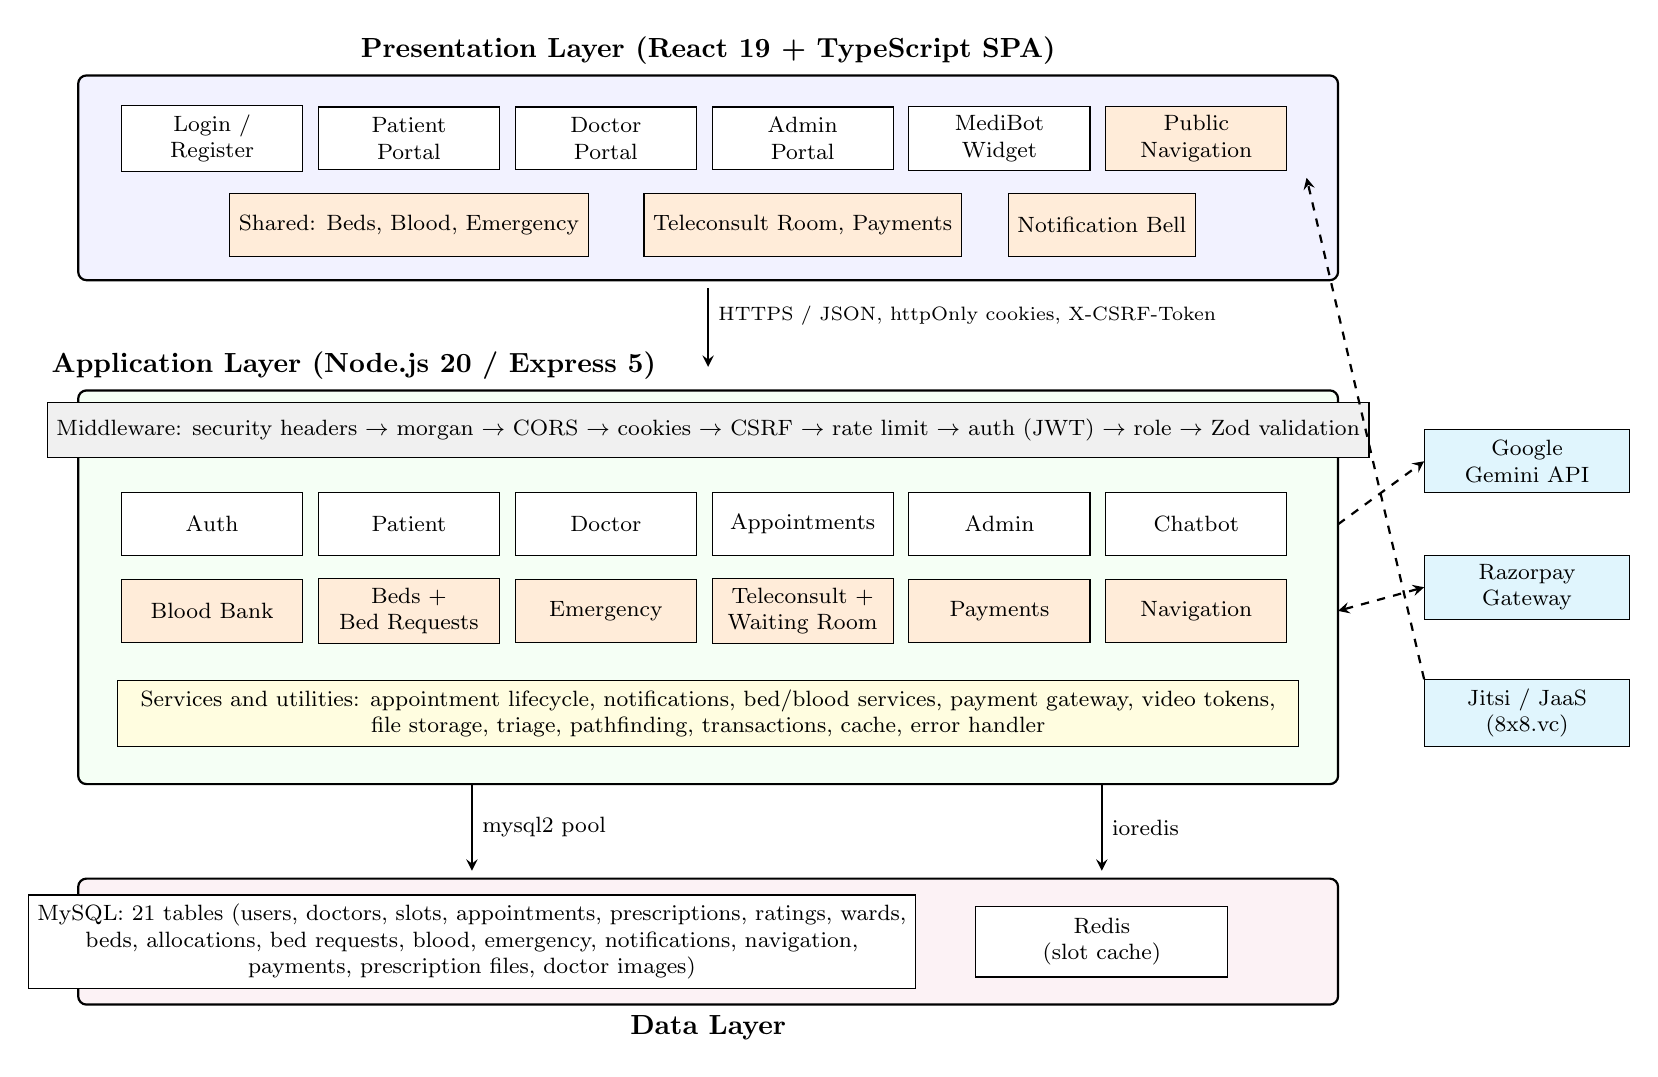
\begin{tikzpicture}[
    font=\footnotesize,
    layer/.style={draw, rectangle, thick, rounded corners=3pt, minimum width=16cm},
    component/.style={draw, rectangle, minimum width=2.3cm, minimum height=0.8cm, align=center, fill=white},
    newc/.style={component, fill=orange!15},
    ext/.style={draw, rectangle, minimum width=2.6cm, minimum height=0.8cm, align=center, fill=cyan!12},
    arrow/.style={->, thick, >=stealth}
]
% Presentation
\node[layer, minimum height=2.6cm, fill=blue!5, label={[font=\bfseries]above:Presentation Layer (React 19 + TypeScript SPA)}] at (0,0) {};
\node[component] at (-6.3,0.5) {Login /\\Register};
\node[component] at (-3.8,0.5) {Patient\\Portal};
\node[component] at (-1.3,0.5) {Doctor\\Portal};
\node[component] at (1.2,0.5) {Admin\\Portal};
\node[component] at (3.7,0.5) {MediBot\\Widget};
\node[newc] at (6.2,0.5) {Public\\Navigation};
\node[newc] at (-3.8,-0.6) {Shared: Beds, Blood, Emergency};
\node[newc] at (1.2,-0.6) {Teleconsult Room, Payments};
\node[newc] at (5.0,-0.6) {Notification Bell};

\draw[arrow] (0,-1.4) -- (0,-2.4) node[pos=0.35, right, font=\scriptsize] {HTTPS / JSON, httpOnly cookies, X-CSRF-Token};

% Application
\node[layer, minimum height=5.0cm, fill=green!4, label={[font=\bfseries, xshift=-4.5cm]above:Application Layer (Node.js 20 / Express 5)}] at (0,-5.2) {};
\node[draw, rectangle, minimum width=15cm, minimum height=0.7cm, fill=gray!12] at (0,-3.2)
{Middleware: security headers $\rightarrow$ morgan $\rightarrow$ CORS $\rightarrow$ cookies $\rightarrow$ CSRF $\rightarrow$ rate limit $\rightarrow$ auth (JWT) $\rightarrow$ role $\rightarrow$ Zod validation};
\node[component] at (-6.3,-4.4) {Auth};
\node[component] at (-3.8,-4.4) {Patient};
\node[component] at (-1.3,-4.4) {Doctor};
\node[component] at (1.2,-4.4) {Appointments};
\node[component] at (3.7,-4.4) {Admin};
\node[component] at (6.2,-4.4) {Chatbot};
\node[newc] at (-6.3,-5.5) {Blood Bank};
\node[newc] at (-3.8,-5.5) {Beds +\\Bed Requests};
\node[newc] at (-1.3,-5.5) {Emergency};
\node[newc] at (1.2,-5.5) {Teleconsult +\\Waiting Room};
\node[newc] at (3.7,-5.5) {Payments};
\node[newc] at (6.2,-5.5) {Navigation};
\node[draw, rectangle, minimum width=15cm, minimum height=0.7cm, fill=yellow!12, align=center] at (0,-6.8)
{Services and utilities: appointment lifecycle, notifications, bed/blood services, payment gateway, video tokens,\\ file storage, triage, pathfinding, transactions, cache, error handler};

\draw[arrow] (-3,-7.7) -- (-3,-8.8) node[midway, right] {mysql2 pool};
\draw[arrow] (5,-7.7) -- (5,-8.8) node[midway, right] {ioredis};

% Data
\node[layer, minimum height=1.6cm, fill=purple!5, label={[font=\bfseries]below:Data Layer}] at (0,-9.7) {};
\node[draw, rectangle, minimum width=9.5cm, minimum height=0.9cm, fill=white, align=center] at (-3,-9.7) {MySQL: 21 tables (users, doctors, slots, appointments, prescriptions, ratings, wards,\\ beds, allocations, bed requests, blood, emergency, notifications, navigation,\\ payments, prescription files, doctor images)};
\node[draw, rectangle, minimum width=3.2cm, minimum height=0.9cm, fill=white, align=center] at (5,-9.7) {Redis\\(slot cache)};

% External
\node[ext] (gem) at (10.4,-3.6) {Google\\Gemini API};
\node[ext] (rzp) at (10.4,-5.2) {Razorpay\\Gateway};
\node[ext] (jit) at (10.4,-6.8) {Jitsi / JaaS\\(8x8.vc)};
\draw[arrow, dashed] (8.0,-4.4) -- (gem.west);
\draw[arrow, dashed, <->] (8.0,-5.5) -- (rzp.west);
\draw[arrow, dashed] (jit.north west) -- (7.6,0.0);
\end{tikzpicture}%
}
\caption{Three-Tier Architecture of Care \& Cure HMS}
\label{fig:arch_ieee}
\end{figure}

Components shaded orange in Figure~\ref{fig:arch_ieee} were added in the second phase. The video call is loaded by the browser directly from JaaS; the backend only decides whether a user may join, keeps the patient in the waiting room until the doctor admits them, and signs the token that opens the room.

\FloatBarrier
\section{Data Flow Diagrams}

\subsection{Level 0 DFD (Context Diagram)}

The Level 0 DFD, shown in Figure~\ref{fig:dfd0}, depicts the system as a single process interacting with seven external entities: Patient, Doctor, Administrator, Visitor, and three external services (Gemini AI, Razorpay and the JaaS video service).

\begin{figure}[H]
\centering
\resizebox{\textwidth}{!}{%
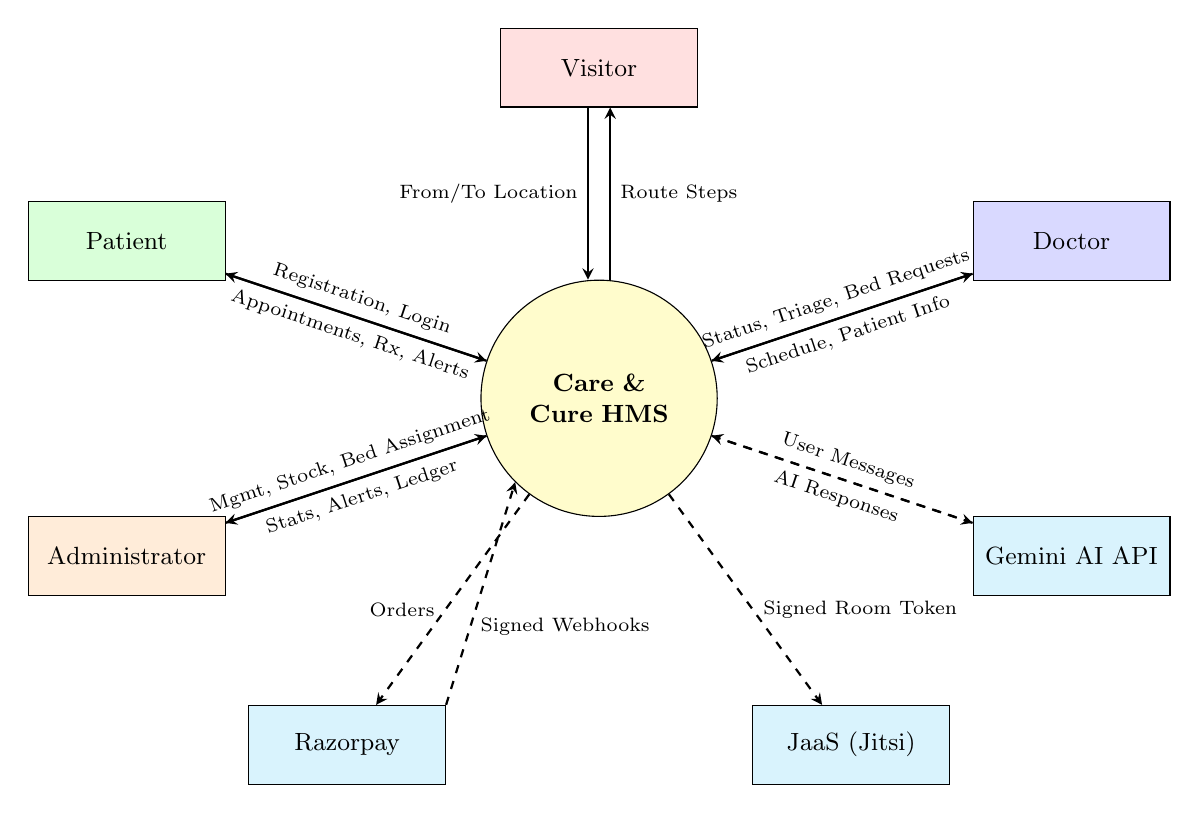
\begin{tikzpicture}[node distance=2cm, font=\small, arrow/.style={thick,->,>=stealth}]

% Central process
\node[draw, circle, fill=yellow!20, minimum size=3cm, text centered, text width=2.5cm] (sys) at (0,0) {\textbf{Care \& Cure HMS}};

% External entities
\node[draw, rectangle, fill=green!15, minimum width=2.5cm, minimum height=1cm, text centered] (pat) at (-6, 2) {Patient};
\node[draw, rectangle, fill=blue!15, minimum width=2.5cm, minimum height=1cm, text centered] (doc) at (6, 2) {Doctor};
\node[draw, rectangle, fill=orange!15, minimum width=2.5cm, minimum height=1cm, text centered] (adm) at (-6, -2) {Administrator};
\node[draw, rectangle, fill=cyan!15, minimum width=2.5cm, minimum height=1cm, text centered] (ai) at (6, -2) {Gemini AI API};

% Patient flows
\draw[arrow] (pat) -- node[above, sloped, font=\scriptsize]{Registration, Login} (sys);
\draw[arrow] (sys) -- node[below, sloped, font=\scriptsize]{Appointments, Rx, Alerts} (pat);

% Doctor flows
\draw[arrow] (doc) -- node[above, sloped, font=\scriptsize]{Status, Triage, Bed Requests} (sys);
\draw[arrow] (sys) -- node[below, sloped, font=\scriptsize]{Schedule, Patient Info} (doc);

% Admin flows
\draw[arrow] (adm) -- node[above, sloped, font=\scriptsize]{Mgmt, Stock, Bed Assignment} (sys);
\draw[arrow] (sys) -- node[below, sloped, font=\scriptsize]{Stats, Alerts, Ledger} (adm);

% AI flows
\draw[arrow, dashed] (sys) -- node[above, sloped, font=\scriptsize]{User Messages} (ai);
\draw[arrow, dashed] (ai) -- node[below, sloped, font=\scriptsize]{AI Responses} (sys);

% Phase-2 entities
\node[draw, rectangle, fill=red!12, minimum width=2.5cm, minimum height=1cm, text centered] (vis) at (0, 4.2) {Visitor};
\node[draw, rectangle, fill=cyan!15, minimum width=2.5cm, minimum height=1cm, text centered] (rzp) at (-3.2, -4.4) {Razorpay};
\node[draw, rectangle, fill=cyan!15, minimum width=2.5cm, minimum height=1cm, text centered] (jit) at (3.2, -4.4) {JaaS (Jitsi)};
\draw[arrow] ([xshift=-4pt]vis.south) -- node[left, font=\scriptsize]{From/To Location} ([xshift=-4pt]sys.north);
\draw[arrow] ([xshift=4pt]sys.north) -- node[right, font=\scriptsize]{Route Steps} ([xshift=4pt]vis.south);
\draw[arrow, dashed] (sys) -- node[left, font=\scriptsize, pos=0.55]{Orders} (rzp);
\draw[arrow, dashed] (rzp.north east) -- node[right, font=\scriptsize, pos=0.35]{Signed Webhooks} (sys.south west);
\draw[arrow, dashed] (sys) -- node[right, font=\scriptsize, pos=0.55]{Signed Room Token} (jit);

\end{tikzpicture}%
}
\caption{Level 0 Data Flow Diagram (Context Diagram)}
\label{fig:dfd0}
\end{figure}

\subsection{Level 1 DFD}

The Level 1 DFD in Figure~\ref{fig:dfd1} decomposes the system into six major processes with their associated data stores and flows.

\begin{figure}[H]
\centering
\resizebox{\textwidth}{!}{%
\begin{tikzpicture}[
  process/.style={
    rectangle, draw=black, rounded corners=2pt,
    minimum width=3.0cm, minimum height=1.3cm,
    align=center, fill=blue!10,
    font=\scriptsize\bfseries, inner sep=4pt
  },
  store/.style={
    rectangle, draw=black, double, double distance=1pt,
    minimum width=3.2cm, minimum height=0.65cm,
    align=center, font=\scriptsize, inner sep=3pt
  },
  ext/.style={
    rectangle, draw=black,
    minimum width=2.2cm, minimum height=0.75cm,
    align=center, font=\scriptsize\bfseries, fill=gray!15
  },
  arr/.style={->, >=stealth, thin},
  lbl/.style={font=\scriptsize, inner sep=1.5pt, fill=white}
]
\node[ext] (pat) at ( 3.0, 17.5) {Patient};
\node[ext] (adm) at ( 8.5, 17.5) {Admin};
\node[ext] (doc) at (14.0, 17.5) {Doctor};
\node[process] (p1) at ( 5.0, 14.0) {P1\\Authentication};
\node[process] (p3) at (12.0, 14.0) {P3\\Prescription\\Management};
\node[process] (p2) at ( 5.0,  9.5) {P2\\Appointment\\Management};
\node[process] (p4) at (12.0,  9.5) {P4\\Slot\\Management};
\node[process] (p5) at ( 5.0,  5.0) {P5\\Chatbot\\Processing};
\node[process] (p6) at (12.0,  5.0) {P6\\Rating\\Management};
\node[store] (ds1) at ( 0.5, 14.65) {D1: Users DB};
\node[store] (ds2) at ( 0.5, 13.35) {D2: Doctors DB};
\node[store] (ds6) at ( 0.5,  2.5)  {D6: Ratings DB};
\node[store] (ds4) at (17.5, 14.65) {D4: Appts DB};
\node[store] (ds5) at (17.5, 13.35) {D5: Prescriptions DB};
\node[store] (ds3) at (17.5,  9.5)  {D3: Slots DB};
\draw[arr] (pat.south)--(3.0,16.6)--(5.0,16.6)--node[lbl,right=2pt]{Credentials}(p1.north);
\draw[arr] (p1.north)--(5.0,16.1)--(3.0,16.1)--node[lbl,above=1pt]{JWT Token}(pat.south);
\draw[arr] (adm.south)--(8.5,15.5)--(5.2,15.5)--node[lbl,above=1pt]{Admin Credentials}(p1.north);
\draw[arr] (doc.south)--(14.0,16.6)--(12.0,16.6)--node[lbl,above=1pt]{Prescription File}(p3.north);
\draw[arr] (p3.north)--(12.0,16.1)--(14.0,16.1)--node[lbl,above=1pt]{Prescription File}(doc.south);
\draw[arr] (doc.south)--(14.0,12.6)--node[lbl,above=1pt]{Doctor Credentials}(6.5,12.6)--(p1.east);
\draw[arr] (pat.west)--(-1.0,17.5)--(-1.0,9.5)--node[lbl,above=1pt]{Book Request}(p2.west);
\draw[arr] (pat.west)--(-2.2,17.5)--(-2.2,5.0)--node[lbl,above=1pt]{Message}(p5.west);
\draw[arr] (pat.west)--(-3.4,17.5)--(-3.4,5.0)--node[lbl,above=1pt]{Feedback}(p6.west);
\draw[arr] (doc.east)--(19.5,17.5)--(19.5,8.3)--(5.0,8.3)--node[lbl,right=2pt]{Status Update}(p2.south);
\draw[arr] (p6.north)--(12.0,18.7)--(8.5,18.7)--node[lbl,above=1pt]{Show Rating}(adm.north);
\draw[arr] ([yshift=3pt]p1.west)--(2.2,14.3)--(2.2,14.65)--node[lbl,above=1pt]{R/W User}(ds1.east);
\draw[arr] ([yshift=-3pt]p1.west)--(2.2,13.7)--(2.2,13.35)--node[lbl,below=1pt]{Read Role}(ds2.east);
\draw[arr] ([yshift=3pt]p3.east)--(15.8,14.3)--(15.8,14.65)--node[lbl,above=1pt]{R/W Appt}(ds4.west);
\draw[arr] ([yshift=-3pt]p3.east)--(15.8,13.7)--(15.8,13.35)--node[lbl,below=1pt]{Write Pres.}(ds5.west);
\draw[arr] (p2.east)--(15.3,9.5)--(15.3,10.1)--node[lbl,above=1pt]{Lock Slot}($(ds3.west)+(0,+0.35)$);
\draw[arr] (p4.east)--node[lbl,above=1pt]{Generate Slots}(ds3.west);
\draw[arr] (p5.east)--(20.5,5.0)--(20.5,9.15)--node[lbl,right=3pt]{Read Slots/Appts}($(ds3.west)+(0,-0.35)$);
\draw[arr] (p6.west)--(10.5,2.5)--(2.1,2.5)--node[lbl,pos=0.35,above=1pt]{Write Rating}(ds6.east);
\draw[arr] (ds6.south)--(0.5,1.4)--(12.0,1.4)--node[lbl,above=1pt]{Fetch Rating}(p6.south);
\end{tikzpicture}%
}
\caption{Level-1 Data Flow Diagram}
\label{fig:dfd1}
\end{figure}

\subsection{Level 1 DFD for the Enhanced Modules}

Figure~\ref{fig:dfd1b} decomposes the processes added in this phase. Doctors send bed and discharge requests to P8, which the administrator fulfils, and the emergency process P9 raises its admissions as emergency bed requests. Every process that changes clinical state also writes to the notifications store (D13), which is read by the notification bell of each user.

\begin{figure}[H]
\centering
\resizebox{\textwidth}{!}{%
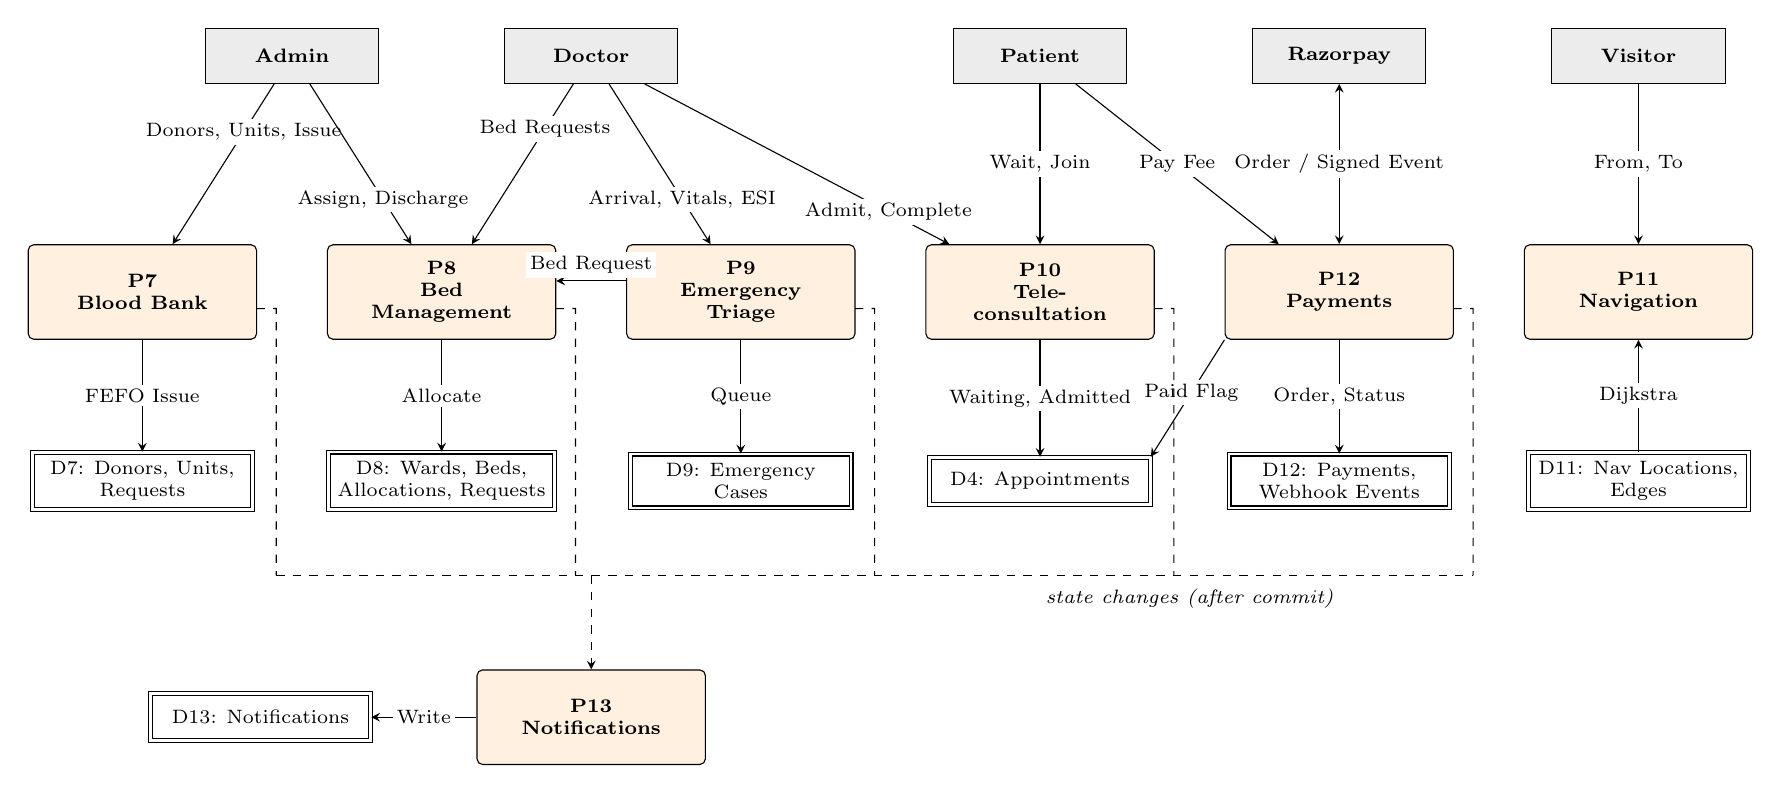
\begin{tikzpicture}[
  process/.style={rectangle, draw=black, rounded corners=2pt, minimum width=2.9cm, minimum height=1.2cm, align=center, fill=orange!12, font=\scriptsize\bfseries},
  store/.style={rectangle, draw=black, double, double distance=1pt, minimum width=2.8cm, minimum height=0.6cm, align=center, font=\scriptsize},
  ext/.style={rectangle, draw=black, minimum width=2.2cm, minimum height=0.7cm, align=center, font=\scriptsize\bfseries, fill=gray!15},
  arr/.style={->, >=stealth, thin},
  bus/.style={dashed, thin},
  lbl/.style={font=\scriptsize, inner sep=1.5pt, fill=white}
]
% externals
\node[ext] (adm) at (1.9,9) {Admin};
\node[ext] (doc) at (5.7,9) {Doctor};
\node[ext] (pat) at (11.4,9) {Patient};
\node[ext] (rzp) at (15.2,9) {Razorpay};
\node[ext] (vis) at (19,9) {Visitor};
% processes
\node[process] (p7)  at (0,6)    {P7\\Blood Bank};
\node[process] (p8)  at (3.8,6)  {P8\\Bed\\Management};
\node[process] (p9)  at (7.6,6)  {P9\\Emergency\\Triage};
\node[process] (p10) at (11.4,6) {P10\\Tele-\\consultation};
\node[process] (p12) at (15.2,6) {P12\\Payments};
\node[process] (p11) at (19,6)   {P11\\Navigation};
% stores
\node[store] (d7)  at (0,3.6)    {D7: Donors, Units,\\Requests};
\node[store] (d8)  at (3.8,3.6)  {D8: Wards, Beds,\\Allocations, Requests};
\node[store] (d9)  at (7.6,3.6)  {D9: Emergency\\Cases};
\node[store] (d4)  at (11.4,3.6) {D4: Appointments};
\node[store] (d12) at (15.2,3.6) {D12: Payments,\\Webhook Events};
\node[store] (d11) at (19,3.6)   {D11: Nav Locations,\\Edges};
\node[process] (p13) at (5.7,0.6) {P13\\Notifications};
\node[store] (d13) at (1.5,0.6) {D13: Notifications};
% external -> process
\draw[arr] (adm) -- node[lbl, pos=0.3]{Donors, Units, Issue} (p7);
\draw[arr] (adm) -- node[lbl, pos=0.72]{Assign, Discharge} (p8);
\draw[arr] (doc) -- node[lbl, pos=0.28]{Bed Requests} (p8);
\draw[arr] (doc) -- node[lbl, pos=0.72]{Arrival, Vitals, ESI} (p9);
\draw[arr] (doc) -- node[lbl, pos=0.8]{Admit, Complete} (p10);
\draw[arr] (pat) -- node[lbl]{Wait, Join} (p10);
\draw[arr] (pat) -- node[lbl, pos=0.5]{Pay Fee} (p12);
\draw[arr, <->] (rzp) -- node[lbl]{Order / Signed Event} (p12);
\draw[arr] (vis) -- node[lbl]{From, To} (p11);
% process -> store
\draw[arr] (p7) -- node[lbl]{FEFO Issue} (d7);
\draw[arr] (p8) -- node[lbl]{Allocate} (d8);
\draw[arr] (p9) -- node[lbl]{Queue} (d9);
\draw[arr] (p10) -- node[lbl]{Waiting, Admitted} (d4);
\draw[arr] (p12) -- node[lbl]{Order, Status} (d12);
\draw[arr] (p12.south west) -- node[lbl, pos=0.45]{Paid Flag} (d4.north east);
\draw[arr] (d11) -- node[lbl]{Dijkstra} (p11);
\draw[arr] ([yshift=4pt]p9.west) -- node[lbl, above=1pt]{Bed Request} ([yshift=4pt]p8.east);
% notification bus
\foreach \x in {0,3.8,7.6,11.4,15.2} {
  \draw[bus] ([yshift=-6pt]\x+1.45,6) -- (\x+1.7,5.79) -- (\x+1.7,2.4);
}
\draw[bus] (1.7,2.4) -- (16.9,2.4);
\node[lbl, font=\scriptsize\itshape] at (13.3,2.1) {state changes (after commit)};
\draw[arr, dashed] (5.7,2.4) -- (p13.north);
\draw[arr] (p13) -- node[lbl]{Write} (d13);
\end{tikzpicture}%
}
\caption{Level-1 Data Flow Diagram of the Enhanced Modules}
\label{fig:dfd1b}
\end{figure}

\FloatBarrier
\section{Database Design}

\subsection{Entity-Relationship Diagram}

The core database comprises six entities with the following relationships and cardinalities. The fifteen tables added in this phase are shown separately in Section~\ref{sec:er-ext}.

\begin{figure}[h]
\centering
\begin{tikzpicture}[
  ent/.style={rectangle, draw=black, minimum width=2.4cm, minimum height=0.9cm,
              align=center, font=\small\bfseries, fill=blue!8},
  rel/.style={diamond, draw=black, aspect=2, minimum width=2.2cm,
              minimum height=0.7cm, align=center, font=\scriptsize, fill=yellow!20},
  att/.style={ellipse, draw=black, minimum width=1.8cm, minimum height=0.55cm,
              align=center, font=\scriptsize},
  pk/.style={ellipse, draw=black, minimum width=1.8cm, minimum height=0.55cm,
             align=center, font=\scriptsize\underbar, text=black},
  lin/.style={-, thick},
  arr/.style={->, >=stealth, thick}
]
  % Entities
  \node[ent] (users)   at (0,   0)    {users};
  \node[ent] (doctors) at (4,   0)    {doctors};
  \node[ent] (slots)   at (8,   0)    {doctor\_slots};
  \node[ent] (appts)   at (4,  -3.5)  {appointments};
  \node[ent] (pres)    at (0,  -6)    {prescriptions};
  \node[ent] (ratings) at (8,  -6)    {ratings};

  % Relationships
  \node[rel] (r1) at (2,  0)    {has};
  \node[rel] (r2) at (6,  0)    {generates};
  \node[rel] (r3) at (0, -2.2)  {books};
  \node[rel] (r4) at (4, -1.8)  {attends};
  \node[rel] (r5) at (6, -1.8)  {uses};
  \node[rel] (r6) at (0, -4.5)  {has};
  \node[rel] (r7) at (8, -4.5)  {receives};

  % users -- has -- doctors  (1:1 for doctor role)
  \draw[lin] (users)   -- node[above]{\scriptsize 1} (r1);
  \draw[lin] (r1)      -- node[above]{\scriptsize 1} (doctors);

  % doctors -- generates -- slots  (1:N)
  \draw[lin] (doctors) -- node[above]{\scriptsize 1} (r2);
  \draw[lin] (r2)      -- node[above]{\scriptsize N} (slots);

  % users(patient) -- books -- appointments  (1:N)
  \draw[lin] (users)   -- node[left]{\scriptsize 1} (r3);
  \draw[lin] (r3)      -- node[right]{\scriptsize N} (appts);

  % doctors -- attends -- appointments  (1:N)
  \draw[lin] (doctors) -- node[left]{\scriptsize 1} (r4);
  \draw[lin] (r4)      -- node[right]{\scriptsize N} (appts);

  % slots -- uses -- appointments  (1:N over time, at most one active)
  \draw[lin] (slots)   -- node[right]{\scriptsize 1} (r5);
  \draw[lin] (r5)      -- node[right]{\scriptsize N} (appts);

  % appointments -- has -- prescriptions  (1:1)
  \draw[lin] (appts)   -- node[left]{\scriptsize 1} (r6);
  \draw[lin] (r6)      -- node[right]{\scriptsize 1} (pres);

  % appointments -- receives -- ratings  (1:1)
  \draw[lin] (appts)   -- node[right]{\scriptsize 1} (r7);
  \draw[lin] (r7)      -- node[right]{\scriptsize 1} (ratings);
\end{tikzpicture}
\caption{Entity-Relationship Diagram of Care \& Cure HMS}
\label{figure:er}
\end{figure}

\subsection{Database Schema}

The following tables specify the full schema for each database entity.

\begin{longtable}{|L{2.8cm}|L{2.6cm}|L{2.2cm}|L{5.2cm}|}
\caption{Schema: \texttt{users} table} \label{tab:users} \\
\hline
\textbf{Column} & \textbf{Type} & \textbf{Constraints} & \textbf{Description} \\
\hline
\endfirsthead
\hline
\textbf{Column} & \textbf{Type} & \textbf{Constraints} & \textbf{Description} \\
\hline
\endhead
\hline
\endfoot
id             & INT              & PK, AUTO\_INC   & Surrogate primary key \\
\hline
name           & VARCHAR(100)     & NOT NULL        & Full name of the user \\
\hline
guardian\_name & VARCHAR(150)     & NULL            & Guardian/relative name \\
\hline
gender         & ENUM             & NULL            & 'male', 'female', 'other' \\
\hline
age            & INT              & NULL            & Age in years \\
\hline
weight         & DECIMAL(5,2)     & NULL            & Body weight in kilograms \\
\hline
medical\_history & TEXT           & NULL            & Free-text prior conditions \\
\hline
phone          & VARCHAR(20)      & NULL            & Contact number \\
\hline
email          & VARCHAR(150)     & UNIQUE NOT NULL & Login identifier \\
\hline
password       & VARCHAR(255)     & NOT NULL        & bcrypt-hashed credential \\
\hline
address        & TEXT             & NULL            & Street address \\
\hline
city           & VARCHAR(100)     & NULL            & City of residence \\
\hline
role           & ENUM             & NOT NULL        & 'patient','doctor','admin' \\
\hline
created\_at    & TIMESTAMP        & DEFAULT NOW()   & Account creation time \\
\hline
\end{longtable}

\begin{longtable}{|L{2.8cm}|L{2.6cm}|L{2.2cm}|L{5.2cm}|}
\caption{Schema: \texttt{doctors} table} \label{tab:doctors} \\
\hline
\textbf{Column} & \textbf{Type} & \textbf{Constraints} & \textbf{Description} \\
\hline
\endfirsthead
\hline
\textbf{Column} & \textbf{Type} & \textbf{Constraints} & \textbf{Description} \\
\hline
\endhead
\hline
\endfoot
id             & INT              & PK, AUTO\_INC   & Doctor-specific key \\
\hline
user\_id       & INT              & FK $\rightarrow$ users(id), UNIQUE, CASCADE & Maps to users table (1-to-1) \\
\hline
specialization & VARCHAR(100)     & NOT NULL        & Medical specialty \\
\hline
fees           & DECIMAL(10,2)    & NOT NULL, DEFAULT 0 & Consultation fee (INR) \\
\hline
rating         & DECIMAL(3,2)     & NOT NULL, DEFAULT 0 & average rating \\
\hline
rating\_count  & INT              & NOT NULL, DEFAULT 0 & Total ratings received \\
\hline
profile\_image & VARCHAR(255)     & NULL            & Version token for the photo URL; bytes in \texttt{doctor\_images} (v2) \\
\hline
\end{longtable}

\begin{longtable}{|L{2.8cm}|L{2.6cm}|L{2.2cm}|L{5.2cm}|}
\caption{Schema: \texttt{doctor\_slots} table} \label{tab:slots} \\
\hline
\textbf{Column} & \textbf{Type} & \textbf{Constraints} & \textbf{Description} \\
\hline
\endfirsthead
\hline
\textbf{Column} & \textbf{Type} & \textbf{Constraints} & \textbf{Description} \\
\hline
\endhead
\hline
\endfoot
id          & INT           & PK, AUTO\_INC     &  primary key \\
\hline
doctor\_id  & INT           & FK $\rightarrow$ doctors(id), CASCADE & Owning doctor \\
\hline
date        & DATE          & NOT NULL          & Calendar date of slot \\
\hline
time        & TIME          & NOT NULL          & Start time (HH:MM:SS) \\
\hline
is\_booked  & TINYINT(1)    & NOT NULL, DEFAULT 0 & 1 if slot is confirmed booked \\
\hline
is\_available & TINYINT(1)  & NOT NULL, DEFAULT 1 & 0 if admin has blocked slot \\
\hline
-- UNIQUE   & (doctor\_id, date, time) & UNIQUE KEY & Prevents duplicate slot rows \\
\hline
\end{longtable}

\begin{longtable}{|L{2.8cm}|L{2.6cm}|L{2.2cm}|L{5.2cm}|}
\caption{Schema: \texttt{appointments} table} \label{tab:appts} \\
\hline
\textbf{Column} & \textbf{Type} & \textbf{Constraints} & \textbf{Description} \\
\hline
\endfirsthead
\hline
\textbf{Column} & \textbf{Type} & \textbf{Constraints} & \textbf{Description} \\
\hline
\endhead
\hline
\endfoot
id          & INT           & PK, AUTO\_INC     &  primary key \\
\hline
patient\_id & INT           & FK $\rightarrow$ users(id)    & Booking patient \\
\hline
doctor\_id  & INT           & FK $\rightarrow$ doctors(id)  & Assigned doctor \\
\hline
slot\_id    & INT           & FK $\rightarrow$ doctor\_slots(id), INDEX & Slot booked (kept after cancellation) \\
\hline
active\_slot\_id & INT     & UNIQUE, NULL      & Equals slot\_id while the visit is live, NULL once cancelled; prevents double-booking (v2) \\
\hline
status      & ENUM          & DEFAULT 'pending' & 'pending','completed','cancelled' \\
\hline
reason      & VARCHAR(255)  & NULL              & Patient-stated reason for visit \\
\hline
consultation\_type & ENUM & DEFAULT 'in\_person' & 'in\_person' or 'video' (v2) \\
\hline
video\_room  & VARCHAR(64)   & UNIQUE, NULL      & Random room name for video visits (v2) \\
\hline
payment\_status & ENUM       & DEFAULT 'unpaid'  & 'unpaid' or 'paid' (v2) \\
\hline
video\_waiting\_at & DATETIME & NULL            & Patient's last poll from the waiting room (v2) \\
\hline
video\_admitted\_at & DATETIME & NULL           & When the doctor admitted the patient (v2) \\
\hline
created\_at & TIMESTAMP     & DEFAULT NOW()     & Booking creation timestamp \\
\hline
\end{longtable}

\begin{longtable}{|L{2.8cm}|L{2.6cm}|L{2.2cm}|L{5.2cm}|}
\caption{Schema: \texttt{prescriptions} table} \label{tab:pres} \\
\hline
\textbf{Column} & \textbf{Type} & \textbf{Constraints} & \textbf{Description} \\
\hline
\endfirsthead
\hline
\textbf{Column} & \textbf{Type} & \textbf{Constraints} & \textbf{Description} \\
\hline
\endhead
\hline
\endfoot
id              & INT           & PK, AUTO\_INC    &  primary key \\
\hline
appointment\_id & INT           & FK $\rightarrow$ appointments(id), UNIQUE & 1 prescription per appointment \\
\hline
doctor\_id      & INT           & FK $\rightarrow$ doctors(id) & Prescribing doctor \\
\hline
patient\_id     & INT           & FK $\rightarrow$ users(id)   & Receiving patient \\
\hline
notes           & TEXT          & NULL             & Doctor's free-text clinical notes \\
\hline
file\_url       & VARCHAR(500)  & NULL             & Access-checked file URL \texttt{/api/\allowbreak files/\allowbreak prescriptions/:id}; bytes in \texttt{prescription\_files} (v2) \\
\hline
created\_at     & TIMESTAMP     & DEFAULT NOW()    & Prescription creation timestamp \\
\hline
\end{longtable}

\begin{longtable}{|L{2.8cm}|L{2.6cm}|L{2.2cm}|L{5.2cm}|}
\caption{Schema: \texttt{ratings} table} \label{tab:ratings} \\
\hline
\textbf{Column} & \textbf{Type} & \textbf{Constraints} & \textbf{Description} \\
\hline
\endfirsthead
\hline
\textbf{Column} & \textbf{Type} & \textbf{Constraints} & \textbf{Description} \\
\hline
\endhead
\hline
\endfoot
id              & INT          & PK, AUTO\_INC   &  primary key \\
\hline
appointment\_id & INT          & FK $\rightarrow$ appointments(id), UNIQUE & One rating per appointment \\
\hline
doctor\_id      & INT          & FK $\rightarrow$ doctors(id) & Rated doctor \\
\hline
patient\_id     & INT          & FK $\rightarrow$ users(id)   & Rating patient \\
\hline
stars           & TINYINT      & CHECK (1--5)     & Integer star score \\
\hline
created\_at     & TIMESTAMP    & DEFAULT NOW()    & Rating submission timestamp \\
\hline
\end{longtable}

The tables added in the second phase are specified below. Columns marked (v2) in the tables above were added to existing tables by migrations.

\begin{longtable}{|L{3.3cm}|L{2.5cm}|L{2.4cm}|L{4.6cm}|}
\caption{Schema: \texttt{wards} table} \label{tab:wards} \\
\hline
\textbf{Column} & \textbf{Type} & \textbf{Constraints} & \textbf{Description} \\
\hline
\endfirsthead
\hline
\textbf{Column} & \textbf{Type} & \textbf{Constraints} & \textbf{Description} \\
\hline
\endhead
\hline
\endfoot
id & INT & PK, AUTO\_INC & Primary key \\
\hline
name & VARCHAR(100) & UNIQUE NOT NULL & Ward name \\
\hline
ward\_type & ENUM & NOT NULL & general, icu, emergency, maternity, pediatric, private \\
\hline
floor & INT & DEFAULT 0 & Floor number \\
\hline
created\_at & TIMESTAMP & DEFAULT NOW() & Creation time \\
\hline
\end{longtable}
\begin{longtable}{|L{3.3cm}|L{2.5cm}|L{2.4cm}|L{4.6cm}|}
\caption{Schema: \texttt{beds} table} \label{tab:beds} \\
\hline
\textbf{Column} & \textbf{Type} & \textbf{Constraints} & \textbf{Description} \\
\hline
\endfirsthead
\hline
\textbf{Column} & \textbf{Type} & \textbf{Constraints} & \textbf{Description} \\
\hline
\endhead
\hline
\endfoot
id & INT & PK, AUTO\_INC & Primary key \\
\hline
ward\_id & INT & FK $\rightarrow$ wards(id), CASCADE & Owning ward \\
\hline
bed\_number & VARCHAR(20) & NOT NULL & Label such as ICU-03 \\
\hline
status & ENUM & DEFAULT 'available' & available, occupied, maintenance, reserved \\
\hline
daily\_rate & DECIMAL(10,2) & DEFAULT 0 & Charge per day (INR) \\
\hline
-- UNIQUE & (ward\_id, bed\_number) & UNIQUE KEY & No duplicate labels in a ward \\
\hline
\end{longtable}
\begin{longtable}{|L{3.3cm}|L{2.5cm}|L{2.4cm}|L{4.6cm}|}
\caption{Schema: \texttt{bed\_allocations} table} \label{tab:allocs} \\
\hline
\textbf{Column} & \textbf{Type} & \textbf{Constraints} & \textbf{Description} \\
\hline
\endfirsthead
\hline
\textbf{Column} & \textbf{Type} & \textbf{Constraints} & \textbf{Description} \\
\hline
\endhead
\hline
\endfoot
id & INT & PK, AUTO\_INC & Primary key \\
\hline
bed\_id & INT & FK $\rightarrow$ beds(id) & Allocated bed \\
\hline
patient\_id & INT & FK $\rightarrow$ users(id), CASCADE & Admitted patient \\
\hline
allocated\_by & INT & FK $\rightarrow$ users(id), SET NULL & Administrator who assigned the bed \\
\hline
attending\_doctor\_id & INT & FK $\rightarrow$ users(id), SET NULL & Doctor whose request led to the stay; sees it and may request discharge \\
\hline
reason & VARCHAR(255) & NULL & Reason for admission \\
\hline
admitted\_at & DATETIME & DEFAULT NOW() & Admission time \\
\hline
discharged\_at & DATETIME & NULL & NULL while the stay is open \\
\hline
open\_patient\_id & INT & UNIQUE, NULL & Equals patient\_id while open, NULL after discharge \\
\hline
open\_bed\_id & INT & UNIQUE, NULL & Equals bed\_id while open, NULL after discharge \\
\hline
\end{longtable}
\begin{longtable}{|L{3.3cm}|L{2.5cm}|L{2.4cm}|L{4.6cm}|}
\caption{Schema: \texttt{blood\_donors} table} \label{tab:donors} \\
\hline
\textbf{Column} & \textbf{Type} & \textbf{Constraints} & \textbf{Description} \\
\hline
\endfirsthead
\hline
\textbf{Column} & \textbf{Type} & \textbf{Constraints} & \textbf{Description} \\
\hline
\endhead
\hline
\endfoot
id & INT & PK, AUTO\_INC & Primary key \\
\hline
name & VARCHAR(100) & NOT NULL & Donor name \\
\hline
blood\_group & ENUM & NOT NULL, INDEX & A+, A$-$, B+, B$-$, AB+, AB$-$, O+, O$-$ \\
\hline
phone / email & VARCHAR & phone NOT NULL & Contact details \\
\hline
last\_donation\_date & DATE & NULL & Used to enforce the 56-day interval \\
\hline
\end{longtable}
\begin{longtable}{|L{3.3cm}|L{2.5cm}|L{2.4cm}|L{4.6cm}|}
\caption{Schema: \texttt{blood\_units} table} \label{tab:units} \\
\hline
\textbf{Column} & \textbf{Type} & \textbf{Constraints} & \textbf{Description} \\
\hline
\endfirsthead
\hline
\textbf{Column} & \textbf{Type} & \textbf{Constraints} & \textbf{Description} \\
\hline
\endhead
\hline
\endfoot
id & INT & PK, AUTO\_INC & Primary key \\
\hline
donor\_id & INT & FK $\rightarrow$ blood\_donors, SET NULL & Source donor \\
\hline
blood\_group & ENUM & NOT NULL & Group of the unit \\
\hline
component & ENUM & NOT NULL & whole\_blood, packed\_rbc, plasma, platelets \\
\hline
volume\_ml & INT & NOT NULL & Volume in millilitres \\
\hline
collected\_on / expires\_on & DATE & NOT NULL & Expiry computed from component shelf life \\
\hline
status & ENUM & DEFAULT 'available' & available, issued, expired, discarded \\
\hline
request\_id & INT & FK $\rightarrow$ blood\_requests, SET NULL & Request the unit was issued to \\
\hline
-- INDEX & (status, component, blood\_group, expires\_on) & INDEX & Serves the FEFO stock query \\
\hline
\end{longtable}
\begin{longtable}{|L{3.3cm}|L{2.5cm}|L{2.4cm}|L{4.6cm}|}
\caption{Schema: \texttt{blood\_requests} table} \label{tab:bloodreq} \\
\hline
\textbf{Column} & \textbf{Type} & \textbf{Constraints} & \textbf{Description} \\
\hline
\endfirsthead
\hline
\textbf{Column} & \textbf{Type} & \textbf{Constraints} & \textbf{Description} \\
\hline
\endhead
\hline
\endfoot
id & INT & PK, AUTO\_INC & Primary key \\
\hline
patient\_id & INT & FK $\rightarrow$ users(id), CASCADE & Recipient \\
\hline
requested\_by & INT & FK $\rightarrow$ users(id), SET NULL & Requesting doctor or admin \\
\hline
blood\_group, component & ENUM & NOT NULL & What is needed \\
\hline
units\_requested & INT & NOT NULL & Number of units \\
\hline
urgency & ENUM & DEFAULT 'routine' & routine, urgent, emergency \\
\hline
status & ENUM & DEFAULT 'pending' & pending, fulfilled, rejected, cancelled \\
\hline
notes & VARCHAR(500) & NULL & Rejection or clinical note \\
\hline
fulfilled\_at & DATETIME & NULL & Time of issue \\
\hline
\end{longtable}
\begin{longtable}{|L{3.3cm}|L{2.5cm}|L{2.4cm}|L{4.6cm}|}
\caption{Schema: \texttt{emergency\_cases} table} \label{tab:ercases} \\
\hline
\textbf{Column} & \textbf{Type} & \textbf{Constraints} & \textbf{Description} \\
\hline
\endfirsthead
\hline
\textbf{Column} & \textbf{Type} & \textbf{Constraints} & \textbf{Description} \\
\hline
\endhead
\hline
\endfoot
id & INT & PK, AUTO\_INC & Primary key \\
\hline
patient\_id & INT & FK $\rightarrow$ users(id), SET NULL & Linked registered patient, if any \\
\hline
patient\_name, age, gender, contact\_phone & mixed & name NOT NULL & Details captured at the door \\
\hline
chief\_complaint & VARCHAR(500) & NOT NULL & Presenting complaint \\
\hline
arrival\_mode & ENUM & DEFAULT 'walk\_in' & walk\_in, ambulance, referral \\
\hline
triage\_level & TINYINT & NOT NULL & ESI level 1 (most urgent) to 5 \\
\hline
heart\_rate, resp\_rate, bp, spo2, temperature & INT / DECIMAL & NULL & Vital signs at triage \\
\hline
status & ENUM & DEFAULT 'waiting' & waiting, in\_treatment, admitted, discharged, transferred \\
\hline
assigned\_doctor\_id & INT & FK $\rightarrow$ doctors(id), SET NULL & Treating doctor \\
\hline
bed\_allocation\_id & INT & FK $\rightarrow$ bed\_allocations, SET NULL & Bed on admission \\
\hline
arrived\_at / closed\_at & DATETIME & arrived NOT NULL & Queue order and closure time \\
\hline
-- INDEX & (status, triage\_level, arrived\_at) & INDEX & Serves the severity-ordered queue \\
\hline
\end{longtable}
\begin{longtable}{|L{3.3cm}|L{2.5cm}|L{2.4cm}|L{4.6cm}|}
\caption{Schema: \texttt{notifications} table} \label{tab:notif} \\
\hline
\textbf{Column} & \textbf{Type} & \textbf{Constraints} & \textbf{Description} \\
\hline
\endfirsthead
\hline
\textbf{Column} & \textbf{Type} & \textbf{Constraints} & \textbf{Description} \\
\hline
\endhead
\hline
\endfoot
id & INT & PK, AUTO\_INC & Primary key \\
\hline
user\_id & INT & FK $\rightarrow$ users(id), CASCADE & Recipient \\
\hline
type & ENUM & NOT NULL & appointment, payment, emergency, blood, bed, teleconsult, system \\
\hline
title / message & VARCHAR & NOT NULL & Content shown in the bell \\
\hline
link & VARCHAR(255) & NULL & In-app route to open \\
\hline
is\_read & TINYINT(1) & DEFAULT 0 & Read flag \\
\hline
-- INDEX & (user\_id, is\_read, created\_at) & INDEX & Unread count and newest-first list \\
\hline
\end{longtable}
\begin{longtable}{|L{3.3cm}|L{2.5cm}|L{2.4cm}|L{4.6cm}|}
\caption{Schema: \texttt{nav\_locations} table} \label{tab:navloc} \\
\hline
\textbf{Column} & \textbf{Type} & \textbf{Constraints} & \textbf{Description} \\
\hline
\endfirsthead
\hline
\textbf{Column} & \textbf{Type} & \textbf{Constraints} & \textbf{Description} \\
\hline
\endhead
\hline
\endfoot
id & INT & PK, AUTO\_INC & Primary key \\
\hline
code & VARCHAR(30) & UNIQUE NOT NULL & Stable code, e.g. MAIN\_ENTRANCE \\
\hline
name & VARCHAR(100) & NOT NULL & Display name \\
\hline
category & ENUM & NOT NULL & entrance, reception, department, ward, facility, elevator, stairs, junction \\
\hline
building / floor & VARCHAR / INT & DEFAULT 'Main' / 0 & Position in the hospital \\
\hline
description & VARCHAR(255) & NULL & Short description \\
\hline
\end{longtable}
\begin{longtable}{|L{3.3cm}|L{2.5cm}|L{2.4cm}|L{4.6cm}|}
\caption{Schema: \texttt{nav\_edges} table} \label{tab:navedge} \\
\hline
\textbf{Column} & \textbf{Type} & \textbf{Constraints} & \textbf{Description} \\
\hline
\endfirsthead
\hline
\textbf{Column} & \textbf{Type} & \textbf{Constraints} & \textbf{Description} \\
\hline
\endhead
\hline
\endfoot
id & INT & PK, AUTO\_INC & Primary key \\
\hline
from\_location\_id, to\_location\_id & INT & FK $\rightarrow$ nav\_locations, CASCADE & Connected locations (UNIQUE pair) \\
\hline
distance\_m & INT & NOT NULL & Walking distance (edge weight) \\
\hline
instruction / reverse\_instruction & VARCHAR(255) & NOT NULL & Directions in each direction \\
\hline
accessible & TINYINT(1) & DEFAULT 1 & 0 if the edge has stairs \\
\hline
\end{longtable}
\begin{longtable}{|L{3.3cm}|L{2.5cm}|L{2.4cm}|L{4.6cm}|}
\caption{Schema: \texttt{payments} table} \label{tab:payments} \\
\hline
\textbf{Column} & \textbf{Type} & \textbf{Constraints} & \textbf{Description} \\
\hline
\endfirsthead
\hline
\textbf{Column} & \textbf{Type} & \textbf{Constraints} & \textbf{Description} \\
\hline
\endhead
\hline
\endfoot
id & INT & PK, AUTO\_INC & Primary key \\
\hline
appointment\_id & INT & UNIQUE, FK $\rightarrow$ appointments, RESTRICT & One payment record per appointment; blocks deleting it \\
\hline
patient\_id & INT & FK $\rightarrow$ users(id), RESTRICT & Payer; blocks deleting the patient \\
\hline
amount\_paise & INT & NOT NULL & Amount in paise, from the doctor's fee \\
\hline
currency & CHAR(3) & DEFAULT 'INR' & Currency \\
\hline
provider & ENUM & NOT NULL & razorpay or mock \\
\hline
provider\_order\_id & VARCHAR(64) & UNIQUE NOT NULL & Gateway order id \\
\hline
provider\_payment\_id & VARCHAR(64) & UNIQUE, NULL & Gateway payment id once paid \\
\hline
status & ENUM & DEFAULT 'created' & created, paid, failed, refund\_due \\
\hline
paid\_at & DATETIME & NULL & Time of capture \\
\hline
\end{longtable}
\begin{longtable}{|L{3.3cm}|L{2.5cm}|L{2.4cm}|L{4.6cm}|}
\caption{Schema: \texttt{payment\_webhook\_events} table} \label{tab:webhook} \\
\hline
\textbf{Column} & \textbf{Type} & \textbf{Constraints} & \textbf{Description} \\
\hline
\endfirsthead
\hline
\textbf{Column} & \textbf{Type} & \textbf{Constraints} & \textbf{Description} \\
\hline
\endhead
\hline
\endfoot
id & INT & PK, AUTO\_INC & Primary key \\
\hline
event\_id & VARCHAR(100) & UNIQUE NOT NULL & Gateway event id; makes webhooks idempotent \\
\hline
event\_type & VARCHAR(60) & NOT NULL & e.g. payment.captured, order.paid \\
\hline
received\_at & TIMESTAMP & DEFAULT NOW() & Receipt time \\
\hline
\end{longtable}
\begin{longtable}{|L{3.3cm}|L{2.5cm}|L{2.4cm}|L{4.6cm}|}
\caption{Schema: \texttt{bed\_requests} table} \label{tab:bedreq} \\
\hline
\textbf{Column} & \textbf{Type} & \textbf{Constraints} & \textbf{Description} \\
\hline
\endfirsthead
\hline
\textbf{Column} & \textbf{Type} & \textbf{Constraints} & \textbf{Description} \\
\hline
\endhead
\hline
\endfoot
id & INT & PK, AUTO\_INC & Primary key \\
\hline
request\_type & ENUM & NOT NULL & admission or discharge \\
\hline
patient\_id & INT & FK $\rightarrow$ users(id), CASCADE & Patient the request is for \\
\hline
requested\_by & INT & FK $\rightarrow$ users(id), SET NULL & Requesting doctor \\
\hline
ward\_type & ENUM & NULL & Preferred ward type (admissions) \\
\hline
allocation\_id & INT & FK $\rightarrow$ bed\_allocations, SET NULL & Stay to end (discharges) \\
\hline
emergency\_case\_id & INT & FK $\rightarrow$ emergency\_cases, SET NULL & Set when raised from the emergency board \\
\hline
urgency & ENUM & DEFAULT 'routine' & routine, urgent, emergency \\
\hline
status & ENUM & DEFAULT 'pending' & pending, fulfilled, rejected, cancelled \\
\hline
reason, admin\_notes & VARCHAR(500) & NULL & Doctor's reason; administrator's note on rejection \\
\hline
open\_key & VARCHAR(40) & UNIQUE, NULL & admission:<patient> or discharge:<allocation> while pending \\
\hline
created\_at, resolved\_at & TIMESTAMP, DATETIME & & Raised and closed times \\
\hline
resolved\_by & INT & FK $\rightarrow$ users(id), SET NULL & Administrator or requester who closed it \\
\hline
\end{longtable}
\begin{longtable}{|L{3.3cm}|L{2.5cm}|L{2.4cm}|L{4.6cm}|}
\caption{Schema: \texttt{prescription\_files} table} \label{tab:presfiles} \\
\hline
\textbf{Column} & \textbf{Type} & \textbf{Constraints} & \textbf{Description} \\
\hline
\endfirsthead
\hline
\textbf{Column} & \textbf{Type} & \textbf{Constraints} & \textbf{Description} \\
\hline
\endhead
\hline
\endfoot
prescription\_id & INT & PK, FK $\rightarrow$ prescriptions, CASCADE & One file per prescription \\
\hline
mime & VARCHAR(50) & NOT NULL & Type detected from the file's first bytes \\
\hline
name & VARCHAR(255) & NOT NULL & Sanitised original file name \\
\hline
size\_bytes & INT & NOT NULL & Size (at most 5~MB) \\
\hline
data & MEDIUMBLOB & NOT NULL & File contents \\
\hline
created\_at & DATETIME & DEFAULT NOW() & Upload time \\
\hline
\end{longtable}
\begin{longtable}{|L{3.3cm}|L{2.5cm}|L{2.4cm}|L{4.6cm}|}
\caption{Schema: \texttt{doctor\_images} table} \label{tab:docimages} \\
\hline
\textbf{Column} & \textbf{Type} & \textbf{Constraints} & \textbf{Description} \\
\hline
\endfirsthead
\hline
\textbf{Column} & \textbf{Type} & \textbf{Constraints} & \textbf{Description} \\
\hline
\endhead
\hline
\endfoot
doctor\_id & INT & PK, FK $\rightarrow$ doctors, CASCADE & One photo per doctor \\
\hline
mime & VARCHAR(50) & NOT NULL & JPEG, PNG or WebP (detected) \\
\hline
data & MEDIUMBLOB & NOT NULL & Image contents (at most 2~MB) \\
\hline
updated\_at & DATETIME & ON UPDATE NOW() & Last change \\
\hline
\end{longtable}


\subsection{Extended Entity-Relationship Diagram}
\label{sec:er-ext}

Figure~\ref{fig:er-ext} shows the fifteen tables added in this phase and how they attach to the core entities (shaded grey). The database therefore grows from six to twenty-one tables. New foreign keys follow three rules: they cascade when the child row has no meaning without its parent (a patient's notifications, a prescription's file), they are set to \texttt{NULL} when the child row is a historical record that must survive (a blood unit whose donor was deleted, a bed request whose doctor left), and they \texttt{RESTRICT} deletion when the child is a financial record (a payment).

\begin{figure}[H]
\centering
\resizebox{\textwidth}{!}{%
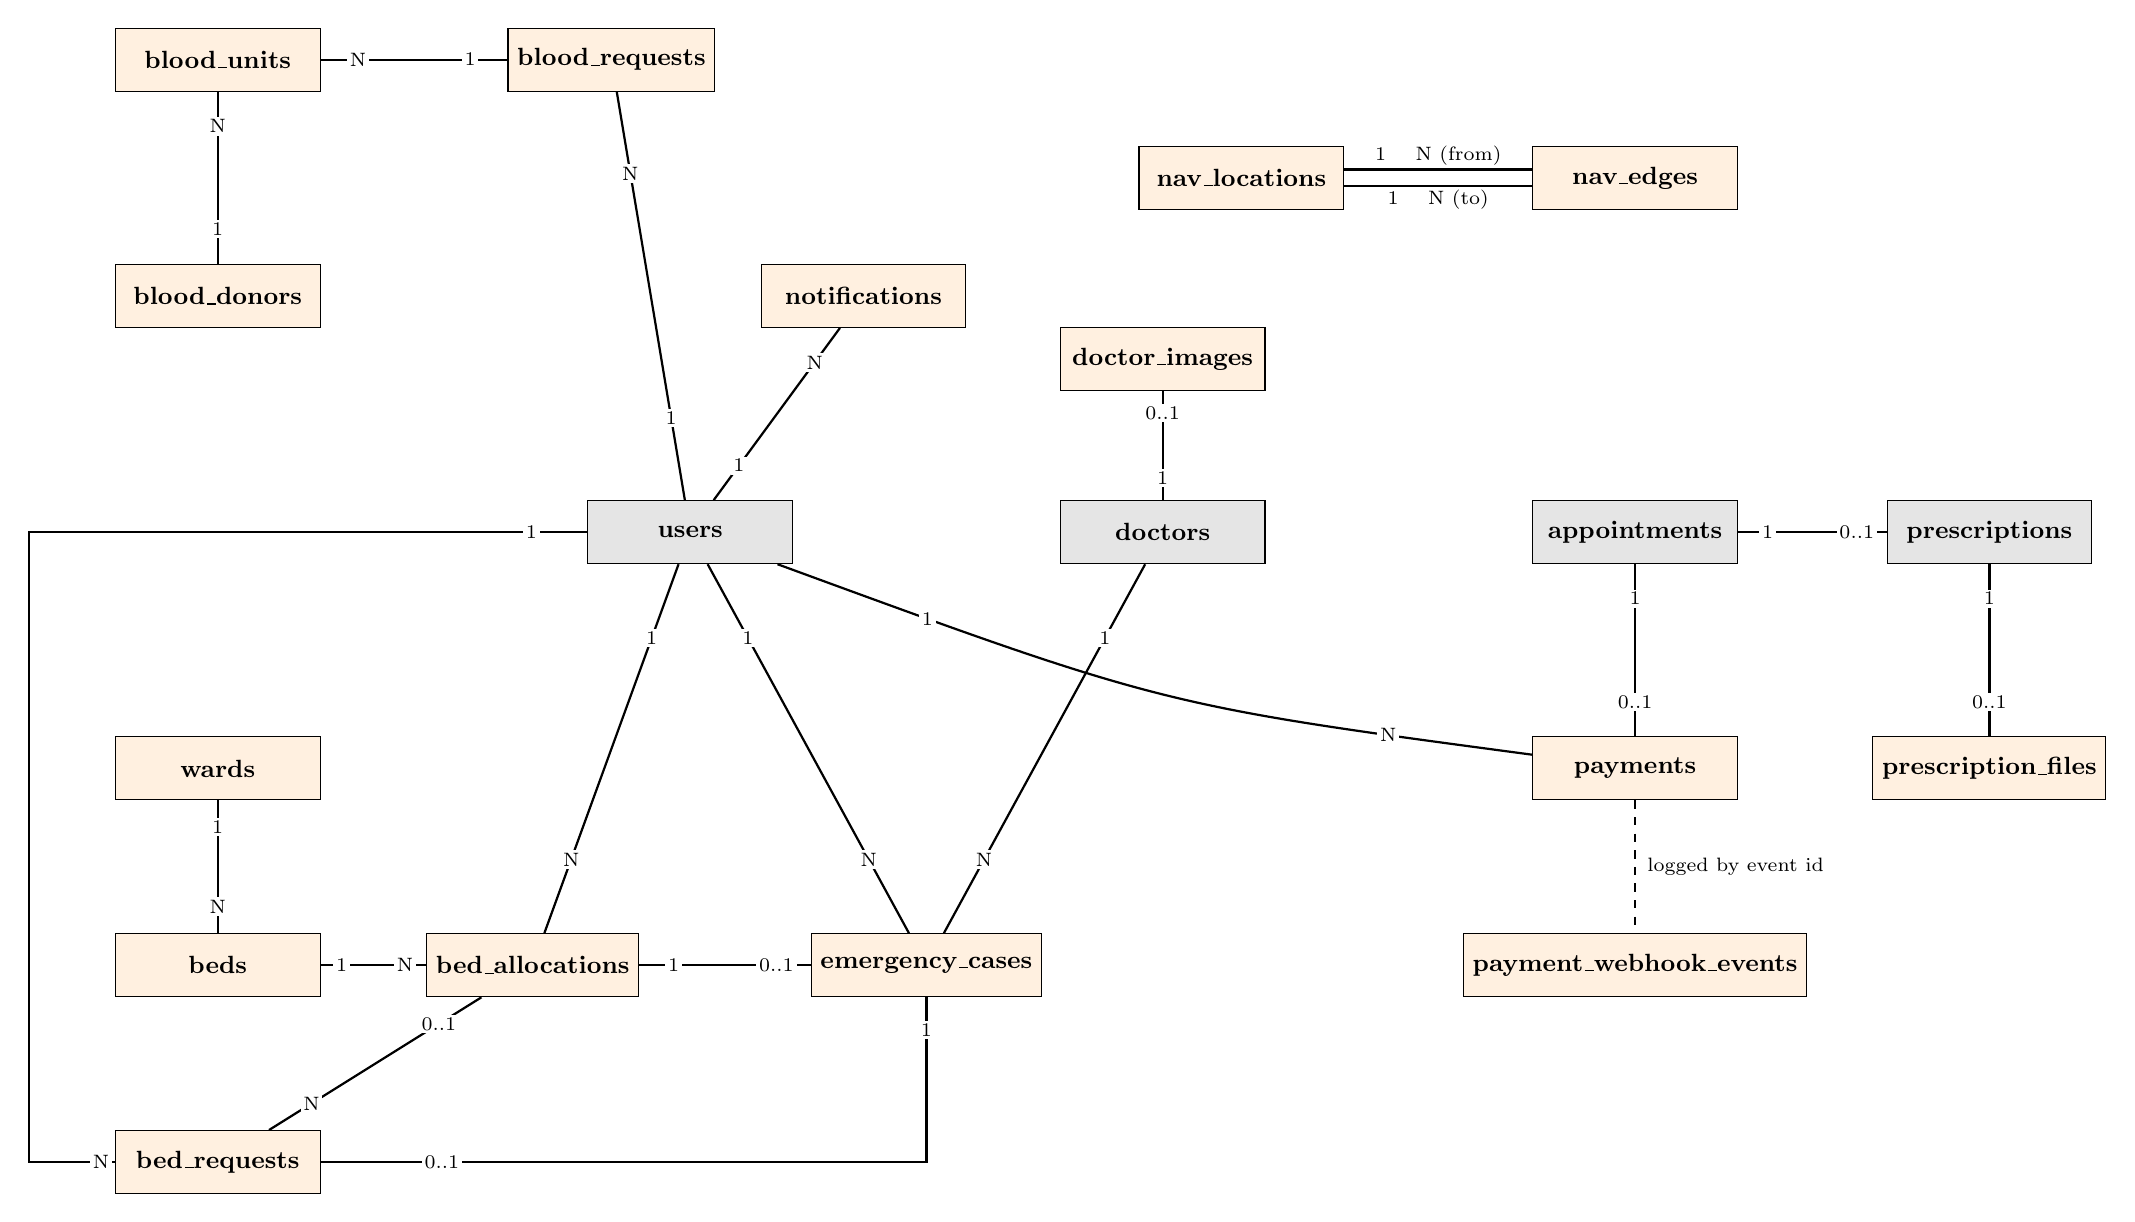
\begin{tikzpicture}[
  ent/.style={rectangle, draw=black, minimum width=2.6cm, minimum height=0.8cm, align=center, font=\small\bfseries, fill=orange!12},
  core/.style={ent, fill=gray!20},
  lin/.style={-, thick},
  card/.style={font=\scriptsize, fill=white, inner sep=1pt}
]
\node[core] (users) at (0,0) {users};
\node[core] (doctors) at (6,0) {doctors};
\node[core] (appts) at (12,0) {appointments};

\node[ent] (wards) at (-6,-3) {wards};
\node[ent] (beds) at (-6,-5.5) {beds};
\node[ent] (alloc) at (-2,-5.5) {bed\_allocations};
\node[ent] (er) at (3,-5.5) {emergency\_cases};
\node[ent] (notif) at (2.2,3) {notifications};
\node[ent] (donors) at (-6,3) {blood\_donors};
\node[ent] (units) at (-6,6) {blood\_units};
\node[ent] (breq) at (-1,6) {blood\_requests};
\node[ent] (pay) at (12,-3) {payments};
\node[ent] (wh) at (12,-5.5) {payment\_webhook\_events};
\node[ent] (loc) at (7,4.5) {nav\_locations};
\node[ent] (bedreq) at (-6,-8) {bed\_requests};
\node[core] (pres) at (16.5,0) {prescriptions};
\node[ent] (pfile) at (16.5,-3) {prescription\_files};
\node[ent] (dimg) at (6,2.2) {doctor\_images};
\node[ent] (edge) at (12,4.5) {nav\_edges};

\draw[lin] (wards) -- node[card,pos=0.2]{1} node[card,pos=0.8]{N} (beds);
\draw[lin] (beds) -- node[card,pos=0.2]{1} node[card,pos=0.8]{N} (alloc);
\draw[lin] (users) -- node[card,pos=0.2]{1} node[card,pos=0.8]{N} (alloc);
\draw[lin] (alloc) -- node[card,pos=0.2]{1} node[card,pos=0.8]{0..1} (er);
\draw[lin] (users) -- node[card,pos=0.2]{1} node[card,pos=0.8]{N} (er);
\draw[lin] (doctors) -- node[card,pos=0.2]{1} node[card,pos=0.8]{N} (er);
\draw[lin] (users) -- node[card,pos=0.2]{1} node[card,pos=0.8]{N} (notif);
\draw[lin] (donors) -- node[card,pos=0.2]{1} node[card,pos=0.8]{N} (units);
\draw[lin] (breq) -- node[card,pos=0.2]{1} node[card,pos=0.8]{N} (units);
\draw[lin] (users) -- node[card,pos=0.2]{1} node[card,pos=0.8]{N} (breq);
\draw[lin] (appts) -- node[card,pos=0.2]{1} node[card,pos=0.8]{0..1} (pay);
\draw[lin] (users) .. controls (6,-2.2) .. node[card,pos=0.15]{1} node[card,pos=0.85]{N} (pay);
\draw[lin, dashed] (pay) -- node[card, right=3pt]{logged by event id} (wh);
\draw[lin] (bedreq) -- node[card,pos=0.2]{N} node[card,pos=0.8]{0..1} (alloc);
\draw[lin] (bedreq.east) -| node[card,pos=0.1]{0..1} node[card,pos=0.9]{1} (er.south);
\draw[lin] (users.west) -- node[card,pos=0.1]{1} (-8.4,0) |- node[card,pos=0.92]{N} (bedreq.west);
\draw[lin] (appts) -- node[card,pos=0.2]{1} node[card,pos=0.8]{0..1} (pres);
\draw[lin] (pres) -- node[card,pos=0.2]{1} node[card,pos=0.8]{0..1} (pfile);
\draw[lin] (doctors) -- node[card,pos=0.2]{1} node[card,pos=0.8]{0..1} (dimg);
\draw[lin] ([yshift=3pt]loc.east) -- node[card,above]{1 \quad N (from)} ([yshift=3pt]edge.west);
\draw[lin] ([yshift=-3pt]loc.east) -- node[card,below]{1 \quad N (to)} ([yshift=-3pt]edge.west);
\end{tikzpicture}%
}
\caption{Extended Entity-Relationship Diagram for the Enhanced Modules}
\label{fig:er-ext}
\end{figure}

\FloatBarrier
\section{Module Design}

\subsection{Authentication Module}

Authentication includes user registration (only for patients) and login for all users. In the first version, a single JSON Web Token was returned to the client, stored in \texttt{localStorage}, and sent in the \texttt{Authorization: Bearer} header. Because any script running on the page can read \texttt{localStorage}, a single cross-site scripting flaw would have exposed every session. In version 2, after a successful login the server issues two tokens and sets them as \emph{httpOnly} cookies that JavaScript cannot read: a short-lived \textbf{access token} (15 minutes, carrying \texttt{id}, \texttt{email}, \texttt{role} and \texttt{type: 'access'}) sent with every request, and a \textbf{refresh token} (7 days, \texttt{type: 'refresh'}) whose cookie path is restricted to \texttt{/api/auth}. When the access token expires, the frontend calls \texttt{POST /api/auth/refresh} once, receives a new pair of tokens (the refresh token is rotated), and retries the original request. \texttt{GET /api/auth/me} restores the session on page reload, and \texttt{POST /api/auth/logout} clears both cookies.

On the server side, the authentication middleware reads the access-token cookie, verifies its signature and expiry with \texttt{jsonwebtoken.verify()}, rejects tokens whose \texttt{type} is not \texttt{access}, and attaches the decoded payload to \texttt{req.user}. Then the \texttt{requireRole(...roles)} middleware checks whether the user's role is one of the roles allowed for the route (several modules, such as emergency, are shared by doctors and administrators). Otherwise, it returns a \texttt{403 Forbidden} response. Because cookies are sent automatically by the browser, every state-changing request must also carry a CSRF token, as described in Section~\ref{sec:security}.

\subsection{Appointment Booking Module}

Here is how the patient books an appointment: (1) patient chooses a specialization and sends a \texttt{GET /api/doctors?specialization=X} request; (2) when choosing a doctor, the patient selects a date, which triggers the request \texttt{GET /api/slots?doctorId=Y\&date=Z}; (3) finally, the patient books a chosen slot by sending \texttt{POST /api/appointments/book} with the JSON body \texttt{\{doctorId, slotId, reason, consultationType\}}, where \texttt{consultationType} is \texttt{in\_person} or \texttt{video}. The slot booking controller wraps these operations in a database transaction in order to avoid any race conditions. Inside the transaction the server also enforces the booking rules: the slot must be free, not blocked and not in the past; the date must lie between today and 13 days ahead; a patient may hold at most five upcoming appointments and at most one with the same doctor on the same day. For a video visit it also generates a random, unguessable room name. After the transaction commits, a confirmation notification is sent to both the patient and the doctor, and the cached availability for that doctor and date is invalidated.

An appointment has a deliberately small life cycle (Figure~\ref{fig:apptstates}): it is \texttt{pending} until it is completed or cancelled, and it can never be reopened. A visit can be completed only from 15 minutes before its start, which is when the video room opens; cancelling frees the slot for another patient and, for a paid visit, marks the payment for refund.

\begin{figure}[H]
\centering
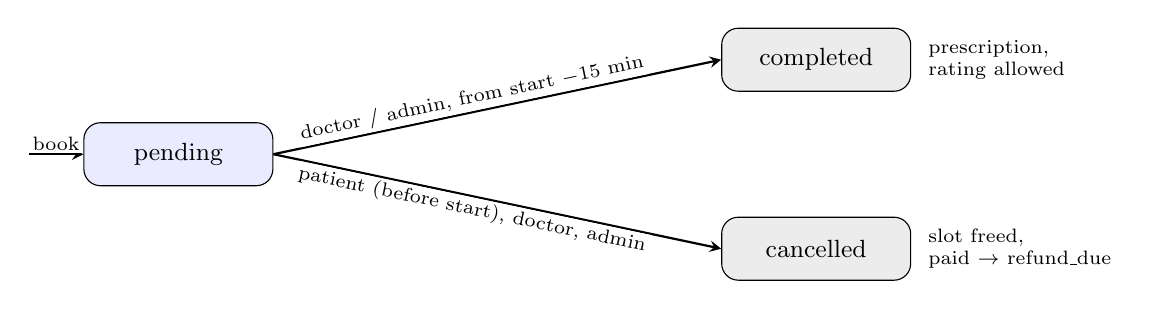
\begin{tikzpicture}[
  st/.style={draw, rounded corners=6pt, minimum width=2.4cm, minimum height=0.8cm, align=center, font=\small, fill=blue!8},
  fin/.style={st, fill=gray!15},
  arr/.style={->, >=stealth, thick},
  lbl/.style={font=\scriptsize, fill=white, inner sep=1pt, align=center}
]
\node[st] (p) at (0,0) {pending};
\node[fin] (c) at (8.1,1.2) {completed};
\node[fin] (x) at (8.1,-1.2) {cancelled};
\draw[arr] (-1.9,0) -- node[lbl, above]{book} (p);
\draw[arr] (p.east) -- node[lbl, sloped, above, pos=0.45]{doctor / admin, from start $-$15 min} (c.west);
\draw[arr] (p.east) -- node[lbl, sloped, below, pos=0.45]{patient (before start), doctor, admin} (x.west);
\node[font=\scriptsize, align=left, anchor=west] at (9.4,-1.2) {slot freed,\\paid $\rightarrow$ refund\_due};
\node[font=\scriptsize, align=left, anchor=west] at (9.4,1.2) {prescription,\\rating allowed};
\end{tikzpicture}
\caption{Appointment Life Cycle}
\label{fig:apptstates}
\end{figure}

\subsection{Slot Generation Module}

The \texttt{generateSlots} function creates 15-minute slots for all the registered doctors from 09:00 to 16:45 (32 slots per day) on a specified date, using \texttt{INSERT IGNORE} with a single multi-row statement so that it is idempotent. The application runs this function when starting up for the next 14 days and schedules it for daily midnight execution via \texttt{node-cron} package. A separate database cleanup query removes past slots that no appointment refers to, in order to prevent \texttt{doctor\_slots} table bloating; a slot that a cancelled appointment still points to is kept, so the visit history stays intact. A failed cleanup is logged and never stops the generation of the next 14 days. Slots are created only inside the booking window, so a request for a date outside it cannot create rows, and blocking a day marks its slots unavailable instead of deleting them, so the midnight generator cannot reopen a blocked day.

\subsection{MediBot AI Chatbot Module}

MediBot is built upon the Gemini 2.5 Flash language model \cite{geminidocs} (Gemini 1.5 Flash in the first version). By means of a specifically crafted system prompt, we constrained the model to perform a limited set of 5 actions: (1) answer general health questions, (2) recommend medical specializations according to symptom descriptions, (3) provide guidance on booking an appointment, (4) provide the information about the hospital and its services, (5) get the patient's appointment history. In the end of the answer, the model provides structured action block \texttt{>>>ACTION:\{"type":XXX\}} that allows triggering corresponding interactions in the UI part. When the patient confirms a booking in the chat, the widget calls the same \texttt{POST /api/appointments/book} endpoint as the booking page and lists only slots that can really be booked, so MediBot is subject to exactly the same rules. The public chat endpoint is rate-limited to 20 messages per minute per client because every message calls a paid external API.

\subsection{Notification Module}

The notification module is a small shared service used by every other module. \texttt{notifyUsers(ids, \{type, title, message, link\})} inserts one row per recipient in a single multi-row statement; \texttt{notifyRoles(roles, ...)} fans a message out to every user of the given roles (for example, an ESI level 1 or 2 arrival alerts every doctor and administrator). Both helpers are deliberately \emph{fire-and-forget safe}: they catch and log their own errors, so that a failure to write a notification can never undo or block the clinical action that triggered it. They are always called \emph{after} the surrounding database transaction has committed, so a notification is never sent for an action that was later rolled back.

\subsection{Enhanced Module Overview}

The seven modules added in this phase follow the same layered pattern as the core: a route file declares the role guards and validation schemas, a controller handles the HTTP request, and a service or utility module holds the business rules so that they can be unit-tested without a database. Their detailed design and implementation are presented in Chapter~\ref{ch:modules}; Table~\ref{tab:modules} gives a summary.

\begin{table}[H]
\centering
\caption{Enhanced Modules: Users, Tables and Core Rules}
\label{tab:modules}
\renewcommand{\arraystretch}{1.25}
\begin{tabular}{|L{2.4cm}|L{2.3cm}|L{3.7cm}|L{5.0cm}|}
\hline
\rowcolor{blue!12}
\textbf{Module} & \textbf{Users} & \textbf{Tables} & \textbf{Core rule} \\
\hline
Blood Bank & Admin (all), Doctor (stock, requests) & blood\_donors, blood\_units, blood\_requests & Compatible units only, exact group first, earliest expiry first; 56-day donor interval \\
\hline
Bed Management & Admin (assign), Doctor (request) & wards, beds, bed\_allocations, bed\_requests & Doctors request, admin assigns; one open allocation per bed and per patient and one pending request of each kind, enforced by unique keys \\
\hline
Emergency & Admin, Doctor & emergency\_cases & ESI level 1--5, queue by level then arrival, fixed status transitions \\
\hline
Teleconsultation & Patient, Doctor & appointments (video columns) & Only the booked pair may join; patient must have paid and waits until the doctor admits; window $-15$ to $+60$ minutes; signed room tokens \\
\hline
Notifications & All signed-in users & notifications & Written after commit; failures never break the triggering action \\
\hline
Navigation & Public (read), Admin (edit) & nav\_locations, nav\_edges & Dijkstra shortest path; accessible mode removes stair edges \\
\hline
Payments & Patient, Admin & payments, payment\_webhook\_events & Amount from DB, HMAC signature check, webhook processed once \\
\hline
\end{tabular}
\end{table}

\FloatBarrier
\section{API Design}

Table~\ref{tab:api} presents the complete REST API endpoint reference for the Care \& Cure HMS. All endpoints return a uniform JSON envelope, \texttt{\{success, data\}} on success and \texttt{\{success: false, message, error: \{code, message\}\}} on failure, so that the frontend handles errors in one place. Path parameters, query strings and bodies are validated by Zod schemas before the controller runs; an invalid request receives \texttt{400} with the list of failing fields.

\begin{longtable}{|L{1.9cm}|L{5.4cm}|L{2.1cm}|L{3.8cm}|}
\caption{REST API Endpoint Reference} \label{tab:api} \\
\hline
\textbf{Method} & \textbf{Endpoint} & \textbf{Auth/Role} & \textbf{Description} \\
\hline
\endfirsthead
\hline
\textbf{Method} & \textbf{Endpoint} & \textbf{Auth/Role} & \textbf{Description} \\
\hline
\endhead
POST & /api/auth/register & Public & Patient self-registration \\
\hline
POST & /api/auth/login & Public & All roles login, returns JWT \\
\hline
GET & /api/patient/profile & Patient & Fetch own profile \\
\hline
PUT & /api/patient/profile & Patient & Update own profile \\
\hline
GET & /api/patient/appointments & Patient & Fetch appointment history \\
\hline
GET & /api/patient/medical-history & Patient & Fetch prescription history \\
\hline
POST & /api/patient/rate & Patient & Submit doctor rating \\
\hline
GET & /api/doctors & Public & List doctors by specialization \\
\hline
GET & /api/slots & Public & Get available slots by doctor/date \\
\hline
POST & /api/appointments/book & Patient & Book a slot \\
\hline
GET & /api/doctor/appointments & Doctor & Doctor's appointment list \\
\hline
GET & /api/doctor/dashboard & Doctor & Dashboard stats \\
\hline
PUT & /api/doctor/appointment-status & Doctor & Update appointment status \\
\hline
POST & /api/doctor/prescription & Doctor & Upload prescription \\
\hline
POST & /api/doctor/slots & Doctor & Create additional slots \\
\hline
GET & /api/admin/users & Admin & List users (v2: server-side search, sort, paging) \\
\hline
POST & /api/admin/doctors & Admin & Create doctor account \\
\hline
PATCH & /api/admin/doctors/:id & Admin & Update doctor details \\
\hline
DELETE & /api/admin/user/:id & Admin & Delete a user \\
\hline
GET & /api/admin/appointments & Admin & List appointments (v2: search, filter, paging) \\
\hline
PATCH & /api/admin/appointments/:id & Admin & Complete or cancel (frees the slot) \\
\hline
DELETE & /api/admin/appointments/:id & Admin & Delete appointment \\
\hline
GET & /api/admin/slots & Admin & View slots by doctor/date \\
\hline
PATCH & /api/admin/slots/:id/toggle & Admin & Toggle slot availability \\
\hline
POST & /api/admin/slots/generate & Admin & Manually trigger slot generation \\
\hline
DELETE & /api/admin/slots/day & Admin & Block a day (slots marked unavailable, not deleted) \\
\hline
POST & /api/chatbot/message & Public & Send message to MediBot \\
\hline
GET & /api/chatbot/doctors & -- & Removed in v2; MediBot uses /api/doctors \\
\hline
GET & /api/chatbot/slots & -- & Removed in v2; MediBot uses /api/slots \\
\hline
POST & /api/chatbot/book & -- & Removed in v2; MediBot books through /api/appointments/book \\
\hline
GET & /api/chatbot/appointments & Patient & View appointments via chatbot \\
\hline
\rowcolor{orange!12} \multicolumn{4}{|l|}{\textbf{Endpoints added in version 2}} \\
\hline
POST & /api/auth/refresh & Cookie & Rotate refresh token, new access token \\
\hline
POST & /api/auth/logout & Cookie & Clear session cookies \\
\hline
GET & /api/auth/me & Any role & Current user (session restore) \\
\hline
GET & /api/admin/doctors & Admin & List doctors \\
\hline
PATCH & /api/admin/users/:id & Admin & Update a user \\
\hline
GET & /api/notifications & Any role & List own notifications, unread count \\
\hline
PATCH & /api/notifications/:id/read & Any role & Mark one as read \\
\hline
PATCH & /api/notifications/read-all & Any role & Mark all as read \\
\hline
GET & /api/beds/wards & Admin, Doctor & Wards with occupancy counts \\
\hline
POST & /api/beds/wards & Admin & Create ward \\
\hline
GET & /api/beds/stats & Admin, Doctor & Hospital occupancy statistics \\
\hline
GET & /api/beds & Admin & Bed grid with patients and pending discharge requests \\
\hline
POST & /api/beds & Admin & Create bed \\
\hline
PATCH & /api/beds/:id/status & Admin & Set maintenance/reserved/available \\
\hline
GET & /api/beds/patients/search & Admin, Doctor & Find a patient by name/email/phone \\
\hline
POST & /api/beds/:id/allocate & Admin & Admit patient to bed (answers a pending request) \\
\hline
POST & /api/beds/allocations/:id/discharge & Admin & Discharge and free the bed \\
\hline
GET & /api/beds/my-patients & Doctor & Beds of the doctor's admitted patients \\
\hline
GET, POST & /api/beds/requests & Admin, Doctor & List / raise bed or discharge requests \\
\hline
POST & /api/beds/requests/:id/fulfill & Admin & Assign a bed or discharge \\
\hline
PATCH & /api/beds/requests/:id/reject & Admin & Reject with a reason \\
\hline
PATCH & /api/beds/requests/:id/cancel & Admin, Doctor & Cancel a pending request \\
\hline
GET & /api/blood/inventory & Admin, Doctor & Stock by group and component \\
\hline
GET, POST & /api/blood/donors & Admin & List / register donors \\
\hline
POST & /api/blood/donations & Admin & Record a donation (creates a unit) \\
\hline
GET & /api/blood/units & Admin & List units \\
\hline
PATCH & /api/blood/units/:id/discard & Admin & Discard a unit \\
\hline
GET, POST & /api/blood/requests & Admin, Doctor & List / raise blood requests \\
\hline
POST & /api/blood/requests/:id/fulfill & Admin & Issue compatible units (FEFO) \\
\hline
PATCH & /api/blood/requests/:id/reject & Admin & Reject with a note \\
\hline
PATCH & /api/blood/requests/:id/cancel & Admin, Doctor & Cancel a pending request \\
\hline
GET & /api/emergency/stats & Admin, Doctor & Open cases per ESI level \\
\hline
GET, POST & /api/emergency/cases & Admin, Doctor & Queue / register an arrival \\
\hline
GET, PATCH & /api/emergency/cases/:id & Admin, Doctor & View / update status, level, doctor \\
\hline
POST & /api/emergency/cases/:id/admit & Admin & Admit directly to a bed \\
\hline
POST & /api/emergency/cases/:id/request-bed & Doctor & Emergency bed request for the case \\
\hline
GET & /api/teleconsult/:appointmentId/join & Patient, Doctor & Waiting state, or room and token \\
\hline
GET & /api/teleconsult/:appointmentId/status & Doctor & Is the patient waiting / admitted \\
\hline
POST & /api/teleconsult/:appointmentId/admit & Doctor & Let the waiting patient in \\
\hline
PATCH & /api/teleconsult/:appointmentId/complete & Doctor & Mark video visit completed \\
\hline
GET & /api/navigation/locations & Public & List locations \\
\hline
GET & /api/navigation/route & Public & Shortest / accessible route \\
\hline
POST, DELETE & /api/navigation/locations[/:id] & Admin & Edit locations \\
\hline
POST, DELETE & /api/navigation/edges[/:id] & Admin & Edit connections \\
\hline
POST & /api/payments/orders & Patient & Create or reuse a payment order \\
\hline
POST & /api/payments/verify & Patient & Verify checkout signature \\
\hline
POST & /api/payments/orders/:orderId/fail & Patient & Record a failed attempt \\
\hline
GET & /api/payments/my & Patient & Own payment history \\
\hline
GET & /api/payments & Admin & Paginated ledger with totals \\
\hline
POST & /api/payments/webhook & HMAC & Razorpay webhook (signature-verified) \\
\hline
POST & /api/patient/appointments/:id/cancel & Patient & Cancel before the start time \\
\hline
GET & /api/files/prescriptions/:id & Patient, Doctor & Prescription file (own only, else 404) \\
\hline
GET & /api/files/doctors/:id/image & Public & Doctor photo \\
\hline
GET & /api/health & Public & Liveness and database check \\
\hline
\end{longtable}

\FloatBarrier
\section{Role-Based Access Matrix}

Table~\ref{tab:rbac} summarises which role can perform which action across the platform. It is enforced on the server by the \texttt{requireRole} middleware on each route, and mirrored on the client, where each portal's routes send a user of another role back to their own section and admin-only buttons are hidden; the client-side checks are a convenience, never a security boundary.

\begin{table}[H]
\centering
\caption{Role-Based Access Matrix}
\label{tab:rbac}
\renewcommand{\arraystretch}{1.2}
\begin{tabular}{|L{6.2cm}|C{1.5cm}|C{1.5cm}|C{1.5cm}|C{1.5cm}|}
\hline
\rowcolor{blue!12}
\textbf{Action} & \textbf{Visitor} & \textbf{Patient} & \textbf{Doctor} & \textbf{Admin} \\
\hline
Browse doctors and free slots, chat with MediBot & \checkmark & \checkmark & \checkmark & \checkmark \\
\hline
Indoor navigation (find a route) & \checkmark & \checkmark & \checkmark & \checkmark \\
\hline
Book appointment, rate doctor, view own history & $\times$ & \checkmark & $\times$ & $\times$ \\
\hline
Cancel an appointment & $\times$ & Own, before start & Own & \checkmark \\
\hline
Open a prescription file & $\times$ & Own & Own & $\times$ \\
\hline
Pay consultation fee, view own payments & $\times$ & \checkmark & $\times$ & $\times$ \\
\hline
Join video consultation & $\times$ & Own, paid, after admit & Own, admits & $\times$ \\
\hline
Complete visit, upload prescription (from 15 min before start) & $\times$ & $\times$ & Own & Complete only \\
\hline
Request a bed or a discharge, view own patients' beds & $\times$ & $\times$ & \checkmark & $\times$ \\
\hline
View full bed grid, assign beds, discharge, answer requests & $\times$ & $\times$ & $\times$ & \checkmark \\
\hline
Create wards and beds, change bed status & $\times$ & $\times$ & $\times$ & \checkmark \\
\hline
View blood stock, raise and cancel requests & $\times$ & $\times$ & \checkmark & \checkmark \\
\hline
Manage donors, record donations, issue or reject & $\times$ & $\times$ & $\times$ & \checkmark \\
\hline
Emergency board: register, triage, treat, close & $\times$ & $\times$ & \checkmark & \checkmark \\
\hline
Emergency admission & $\times$ & $\times$ & Request bed & Admit \\
\hline
Edit navigation map, view payment ledger, manage users and slots & $\times$ & $\times$ & $\times$ & \checkmark \\
\hline
Receive in-app notifications & $\times$ & \checkmark & \checkmark & \checkmark \\
\hline
\end{tabular}
\end{table}

\FloatBarrier
\section{Concurrency and Data Integrity Design}

Several workflows in a hospital are naturally concurrent: two receptionists may try to admit patients to the last ICU bed, two patients may click the same slot, or a payment webhook may arrive while the patient's browser is verifying the same payment. The design follows three rules, drawn from classical transaction processing \cite{gray1992}:

\begin{enumerate}
    \item \textbf{Lock the row you are about to change.} Every read-modify-write runs in a transaction that reads the target row with \texttt{SELECT ... FOR UPDATE}. Other transactions that want the same row wait until the first commits, and then see the new state.
    \item \textbf{Always lock in the same order.} Deadlocks happen when two transactions lock the same rows in opposite orders. The documented lock orders are \emph{bed request $\rightarrow$ emergency case $\rightarrow$ bed $\rightarrow$ patient user $\rightarrow$ allocation} for admissions, \emph{appointment $\rightarrow$ payment} for payments, and \emph{appointment $\rightarrow$ slot} for cancellation (booking never holds an appointment lock while it takes a slot). Queries that would also lock a joined row (\texttt{JOIN ... FOR UPDATE}) are split into a locked read and a separate unlocked read. If MySQL still reports a deadlock, the shared \texttt{inTransaction} helper retries the whole transaction up to two times on a fresh connection.
    \item \textbf{Let the database have the last word.} Application checks give friendly error messages, but unique keys guarantee correctness: \texttt{appointments.active\_slot\_id} is unique while a visit is live, \texttt{bed\_requests.open\_key} allows one pending request of each kind, \texttt{payments.appointment\_id} and \texttt{provider\_order\_id} are unique, \texttt{payment\_webhook\_events.event\_id} is unique, and \texttt{bed\_allocations} has unique \texttt{open\_bed\_id} and \texttt{open\_patient\_id} columns. A violated key is translated into a \texttt{409 Conflict} response instead of a server error.
\end{enumerate}

Side effects outside the database, such as notifications and calls to the payment gateway, are never performed inside a transaction, because a retried transaction would repeat them and a long external call would hold locks for its whole duration.
